\documentclass[preprint,nocopyrightspace]{styles/sig-alternate}

% Basic core packages
\usepackage{amsmath}
\usepackage{hyperref}
\usepackage{graphicx}
\usepackage{amssymb}
\usepackage{changepage}
\usepackage{times}
\usepackage{xcolor}
\usepackage{lipsum}% for dummy text

% standard packages that must be loaded after hyperref
\usepackage[auth-lg]{authblk}
\usepackage{bookmark}
\usepackage{booktabs}
\usepackage[final]{listings}
\usepackage{lscape}
\usepackage{mathtools}
\usepackage{paralist}
\usepackage{flushend}

% local packages for references formatting
\usepackage{styles/natbib-cite}
\usepackage{styles/natbib-acm}

% packages that must be loaded after both hyperref and natbib
\usepackage{hypernat}
\usepackage{cleveref}

% Not sure what these are for
\crefname{section}{Section}{Sections}
\crefname{table}{Table}{Tables}
\crefname{figure}{Figure}{Figures}
\crefname{subfigure}{Figure}{Figures}

% For including code
\definecolor{codegreen}{rgb}{0,0.6,.2}
\definecolor{codegray}{rgb}{0.5,0.5,0.5}
\definecolor{codepurple}{rgb}{0.58,0,0.82}
\definecolor{backcolor}{rgb}{0.94,0.94,1}
\definecolor{light-gray}{gray}{0.55}
\lstdefinestyle{small}{
    backgroundcolor=\color{backcolor},   
    commentstyle=\color{codegreen},
    keywordstyle=\color{blue},
    numberstyle=\tiny\color{codegray},
    stringstyle=\color{codepurple},
    basicstyle=\footnotesize,
    breakatwhitespace=false,         
    breaklines=false,                 
    captionpos=b,                    
    keepspaces=false,                 
    numbers=left,                    
    numbersep=5pt,                  
    showspaces=false,                
    showstringspaces=false,
    showtabs=false,                  
    tabsize=4
}

% Header
\title{A Smarter Smart Contract Testing Tester}
\author{
	  Vincent Yang , 	\quad 
      Sahana Mundewadi, \quad
      Joseph Kotlarek,  \quad 
      Doug Sherman  
}
\pagenumbering{arabic}

% Begin Document by linking associated .tex files in order.
\begin{document}
\lstset{style=small}
\maketitle

\begin{abstract}
As the drive for decentralized frameworks based on blockchains such as Bitcoin and Ethereum continues to grow, the need for reliable and accurate Smart Contracts is increasingly important. To this end, testing suites such as Mythril, Oyente, and SmartCheck have been produced that employ static analysis techniques such as symbolic and chain execution. These methods have been shown to vary wildly in which bugs they can detect, and studies have been made to demonstrate the number of bugs each can detect. However, there are minimal studies discussing the relevance of the bugs detected; which is vital when bugs such as the DAO bug can lead to over 60 million in damages. Thus we introduce a novel system for testing smart contracts with both Mythril and Oyente through a user-driven interface. This tool allows the user to specify what parts of the code are most important and emphasize which tests provide the most coverage over these regions. We used these tools to study the DAO Solidity scripts as well as 40 other scripts including \texttt{Honeypot.sol} and \texttt{BrokenToken.sol}. We found that Oyente consistently finds more bugs than Mythril, SmartCheck finds more bugs on smaller contracts, but Mythril finds the most relevant bugs and provides further insight into the source of these bugs. Moreover, the trend between code complexity and bugs is a bimodal trend where the smallest and largest scripts contain the most problems. Overall, we have shown this tool allows users to explore their smart contracts with more control using metrics truly relevant to their search for mistakes. 
\end{abstract}    
\section{Introduction}

Since Bitcoin was first introduced in 2009, decentralized transaction systems have surged in popularity in both the academic and private sectors \cite{nakamoto2008bitcoin}. To maintain decentralization, these systems rely on a consensus ledger maintained solely by the users, and thus no institution is required to maintain it. Blockchains were created as a way to handle the intricacies of a decentralized ledger system for transactions; however, today blockchains are used for much more. Miller et al. demonstrated a way to preserve data using blockchains by incentivizing users to store large volumes of data rather than provide large amount of computing power \cite{miller2014permacoin}, and use cases have been proposed to built entire operating systems from the blockchain structure \cite{factombos,tapscott2016blockchain}. However, with no central force governing these tools, new problems arise to handle secure and trusted transactions, data transfers, and events. \\

Thus, smart contracts were developed to provide a secure way to handle events in decentralized systems. A smart contract follows the success of Bitcoin's consensus ledger by providing a "consensus protocol" that a blockchain decides upon to guarantee any event between two entities is handled without third party intervention and results in costly penalties for any party found in breach of the contract \cite{szabo1997idea, luu2016making,daian2016dao}. These contracts can be used for transactions between two people, allow for digital identities, and facilitate data sharing. An example of a smart contract is shown in figure \ref{code:example}. In this example we have a basic script that sends money only if the condition \texttt{defined\_condition.is\_met()} succeeds. This condition can be any collection of jointly agreed upon requirements, and thus a wide array of contracts can be decentralized using smart contracts. \\

Unfortunately, the current state of smart contract code quality is remarkably dismal. Solidity, the most popular smart contract programming language, was created to be similar to JavaScript and attract as many users as possible \cite{bartolettipompianuanalysis, systematicstudy}. Many developers on Solidity are drawn in by the sensationalized articles of blockchain and ``Hello World'' applications are everywhere to be found. Many developers do not know about the specifics of Solidity and the many pitfalls. One of the biggest pitfalls is that many functions can fail \cite{systematicstudy}. Most notably, the send function -- the function that sends money from one account to another, can fail. When this happens, it is currently the developer's responsibility to roll back what has happened appropriately \cite{luu2016making}. In fact, this has been the cause for many significant attacks on the Ethereum network. \\

\begin{figure}[h!]
\lstinputlisting[language=C]{code/example.txt} 
\label{code:example}
\caption{An example of a smart contract that sends money if a certain condition is met; allowing for many types of contracts.}
\end{figure}

By nature of the blockchain, developing decentralized applications is quite different from that of normal development. Since the blockchain is created to be immutable, patches are issued as new versions of the same program, and everyone is encouraged to switch over. However, the old version of an application or contract is still accessible on the global database, the ledger. Additionally, it takes time for an application to spread throughout the network \cite{luu2016making}. This inability to roll back increases the importance of getting code right on the first try \cite{luu2016making}. \\

Luckily, many researchers have worked to mitigate these attacks by providing code analysis tools. These analysis tools cover a wide variety of bugs and coding styles to promote clean, readable code\cite{atzei2017survey}. Unfortunately, not all of these tools are easy to use and many are poorly documented. This is where our tool comes in play. \\

Our tool works by allowing people to run their code on a variety of testing tools. By making this process as simple as selecting a set of testing suites, the users can easily see what errors are generated by what vulnerabilities and from what testing suite. Additionally, we are working to allow the user to specify code snippets of higher priority so we can rank errors in those regions higher. Another neat benefit is that many of these testing suites are still in active development, so new vulnerabilities would still be caught without any further action from the developer. In the grand scheme, we want to promote code quality and make improving code quality on smart contracts a trivial task. Hopefully this improves the state of smart contracts for the community as a whole. 

\section{Related Work}

Recently, research into removing bugs from smart contracts has surged. This has lead to an array of tools designed to ensure the stability and accuracy of smart contracts. This has lead to three distinct schools of thought in bug detection. One method is Static analysis, where tools rely on techniques that do not require running the code, such as determining any paths that are unreachable \cite{everts2018will}. Code coverage, which is focusing solely on testing as much of a block of code as possible, and linters, a technique designed to preemptively catch bugs during development, account for the remaining tool categories \cite{manticore}. Based off studies from researchers like Kochhar et al., code coverage is known to have little to no correlation with actual bugs \cite{kochhar2017code, zhou2018security}, and linters need to be employed before development; providing no support for the extensive list of smart contracts already in use. Thus, our study focuses primarily on comparing static analysis tools through a wide array of smart contracts. \\

The current smart contract static analysis tools employ a wide variety of techniques to study the code. Mythril, Oyente, and Porosity. Each of these techniques travel branches within the solidity script, studying possible points of failure along the way. Oyente employs symbolic execution, a technique that uses symbols to determine which values traverse certain paths in the code \cite{king1976symbolic}. Mythril provides a comprehensive blockchain exploration tool that has finally allowed chain exploration to succeed in smart contract testing \cite{sen2005cute}. Porosity translates EVM bytecode into Solidity; allowing for static and dynamic analysis of the contracts \cite{porosity}. \\

Fontein studied each of these static analysis techniques in detail. In this study, he found that Oyente detects on average 75\% of the errors, but severely lacks in missed timestamp dependency bugs. Moreover, since Oyente relies on symbolic execution, a missed opportunity to provide an export of the script's control flow graph (CFG) could drastically improve it's effectiveness. Porosity's decompilation tools were shown to be very limited, and this tool only detects re-entrancy bugs. However, many of the re-entrancy bugs it detects are incorrect. Fontein defined Mythril as the clear winner as it detected the most bugs without false positives. However, Fontein did not mention the quality of the bugs, such as fixing the infamous DAO bug that cost almost 60 million in lost funds \cite{fontein2018comparison}. \\

Even with this surge in tools, smart contracts filled with bugs are still being created. This is largely due to the lack of usability within each tool. With the huge opportunity for smart contracts in the financial sectors, many non-technical developers are creating contracts of their own \cite{tapscott2016blockchain}. However, these tools require knowledge of concepts such as EVM bytecode or symbolic execution. Thus, systems have been developed to provide user friendly interfaces to these tools. SmartCheck allows users to run tools on their website with ease, but the analysis is hidden from the user on their backend. Thus, user-driven studies are limited, and focusing analysis on important aspects is difficult \cite{smartcheck}. \\

Thus, we explored these smart contract testing solutions, and validate these tools using novel metrics that consider the bugs unique to blockchain platforms and the security problems presented by these decentralized transactional events. Moreover, we developed a tool for comparing these testing suites on a specific codebase through user-driven studies. This tool combines results of the bugs discovered by the testing suites, and explores developer driven metrics allowing specific blocks of code to be tagged with more importance. This allows developers to compare available testing options on their own codebase with metrics of far more meaning than generic code coverage. With our tool, they have the ability to quickly see potential vulnerabilities in their code. \\




\section{Methods}

\begin{figure*}
\begin{center}
  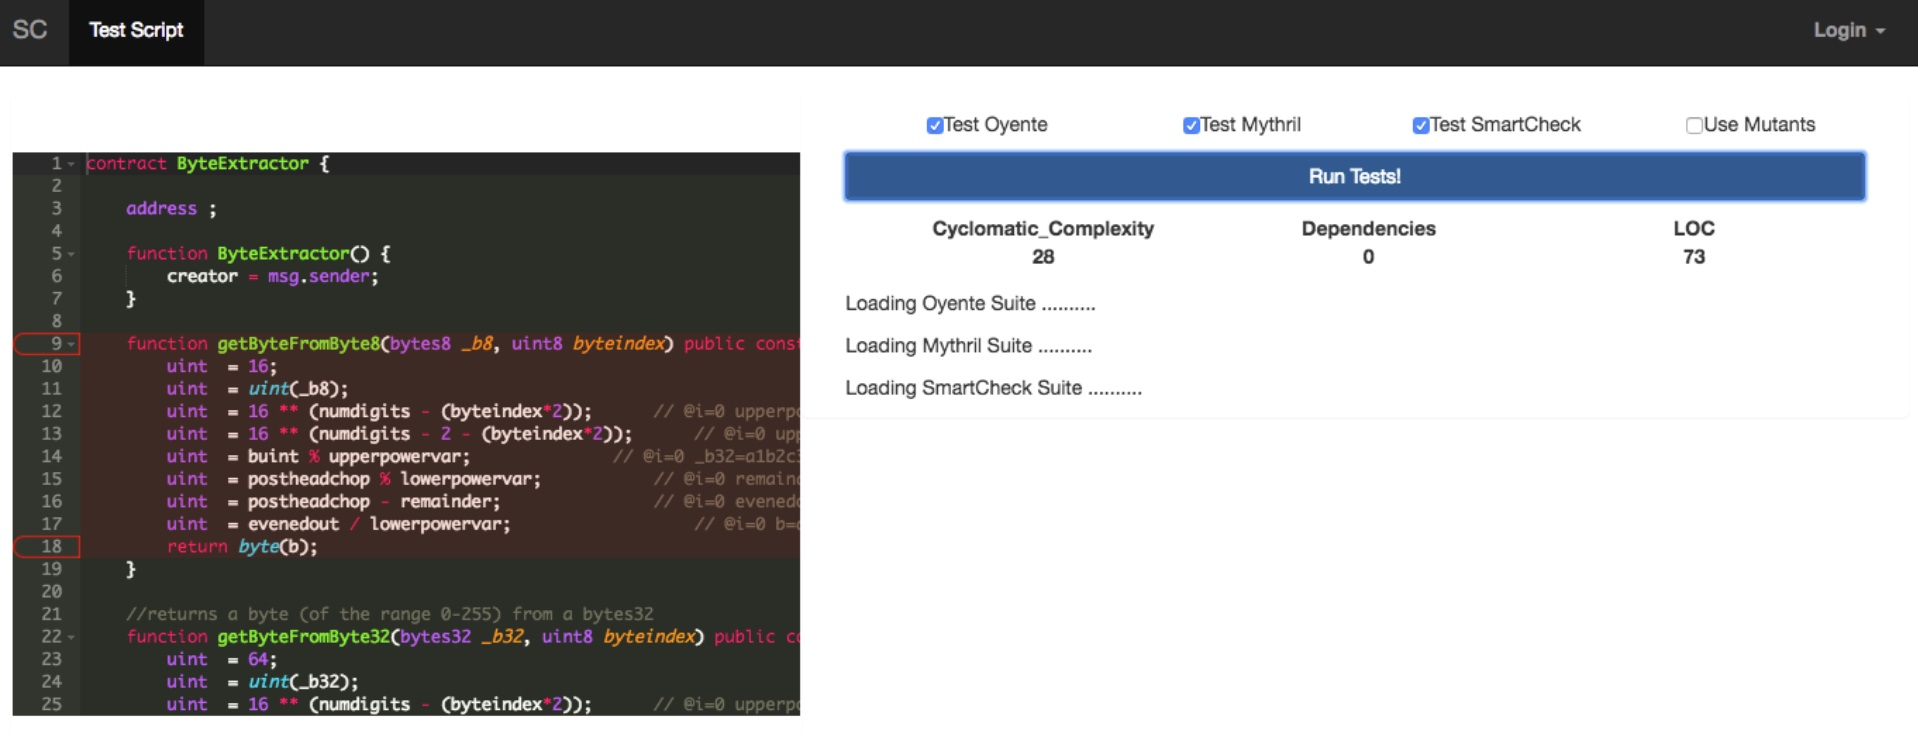
\includegraphics[width=0.9\textwidth]{img/ui1.jpg}
  \label{fig:ui1}
  \caption{The Smarter Smart Contract Testing Tester User Interface}
\end{center}
\end{figure*}

\begin{table}[h!]
%\centering
\begin{tabular}{|cccc|}
\hline
\textbf{Vulnerability}	&\textbf{Oyente}&	\textbf{Mythril} & \textbf{SmartCheck}	\\
\hline
Integer Overflow & yes & yes &  \\
Integer Underflow & yes & yes &  \\
Callstack Depth Attack & yes & yes & \\
Transaction-ordering & yes & yes & yes\\
Re-Entrancy & yes & yes & yes \\
Unprotected Function & & yes & \\
Missing check on return & & yes & \\
Multiple sends & & yes & \\
Complex fallback& & yes & \\
DoS by External Contract & & & yes \\
Gas costly patterns & & & yes \\
Locked Money & & & yes \\
Unchecked external call & & yes & yes \\
Hardcoded address & & & yes \\
Using tx.origin & & yes & yes\\
Costly loop & & & yes \\
Integer division & & & yes \\
Malicious libraries & & & yes \\
Depreciated functions & & yes & \\
\hline
\end{tabular}\\
\label{coverage}
\caption{ Suite coverage of more notable vulnerabilities}
\end{table} 
\subsection{Testing Suites}
\subsection*{Choosing Testing Suites}
While investigating various testing suites, we found that most analysis tools covered similar bugs. As a result, we chose our final testing suites based off of popularity, vulnerability coverage, and ease of use. Out of all analysis tools, Oyente was the most accurate -- it had the lowest false positive/negative rates \cite{ntnutools}. It was also the best for consistency, in that it could analyze source code and bytecode to check for discrepancies. SmartCheck had the widest coverage; its knowledge base is more than double the size of each of the others. Additionally, Oyente, Mythril, and SmartCheck each use a different type of analysis (symbolic, concolic, and static respectively), thus providing a variety of perspectives. Throughout trying other testing suites, many were difficult to set up. They required specific dependencies or operating systems, only worked for certain versions of Solidity, or had an extremely limited feature set. Ultimately, we decided that these three would provide the widest and most accurate coverage for developers using our platform. \\

Furthermore, we found that contracts often violate the same bugs, even if these bugs have induced incredibly expensive errors in the past. As such, these tools' coverages also overlap on the most common bugs. Some examples of these are having integer underflow or overflow, running out of stack frames, re-entrancy, denial of service, being dependent on timestamps or contract execution ordering. Most notably, the re-entrancy attack which was used on the DAO is covered by all three of our testing suites. Other suites we investigated are Manticore, Solgraph, solidity-coverage, Solcheck, Solint, Solium, Solhint, F*, Gasper, and Porosity. Most of these had insignificant coverage or insufficient documentation. A list of our testing suite coverage on the more significant vulnerabilities is in table \ref{coverage} \cite{mythrilvuln, scvuln}. 

\subsubsection{Vulnerability Relevance and Contract Testing}

We chose these bugs because they are well known but still occur in many smart contracts. We checked these vulnerabilities on contracts of all sizes. Some notable contracts are in the repository. The two most well known are Cryptokitties and King of the Ether Throne. Cryptokitties is one of the first blockchain games, where you collect and breed digital cats. Players can breed cats together to create new, unique cats. In December 2017, this game got so popular that it congested the network, causing all time highs in transactions and slow speeds. The most expensive cat bought was 117,712 USD. The Gas limit was even increased in response to Cryptokitties. Next, King of the Ether Throne is a status symbol where you pay a fee to become the king. You must pay more than what the current king previously paid to become the king to knock him off the throne. Yet, there was a vulnerability. By adding a complex fallback that would take a large amount of gas, thus causing the send function to fail, one could claim the throne while not paying the previous king anything. These are both large, well-known contracts, thus giving us a good view into how the tool works with real life contracts.


\subsection*{Oyente}
Oyente works by finding the gap between contract programmers' assumptions about the system and the actual nature of the platform. This gap is the core reason for thousands of bugs on the Ethereum network -- the most popular smart contract platform today. OYENTE uses symbolic execution to analyze Ethereum smart contracts \cite{luu2016making}. \\

As proof of OYENTE's effectiveness, the creators tested 19,366 smart contracts and found that 8,833 contracts have potential bugs. The total value in these contracts was equal to around 30 million USD when they created the tool. Ethereum's value has risen dramatically since. Over the last few years, several vulnerabilities have made headlines worldwide. The most significant of these is TheDAO bug, which had a 60 million loss in USD. If the creators had used OYENTE, they would have caught this bug early on. \\

Some notable bugs Oyente searches for are mishandled exceptions, deliberately hitting the stack limit, timestamp-independent calls, and functions that depend on transaction ordering. The first two are significant because the developer must explicitly implement what happens when a call fails. For instance, in the \texttt{send} function, where people send Ether to someone else, it is fully possible for this function to fail. In response, the developer must revert all that has happened thus far, such as un-withdrawing money from an account. Next, timestamp-independence and transaction ordering are important because miners are allowed to choose what contracts to run. Often times, developers use timestamps as seeds for randomization, but this is easily attacked when miners can determine the seed. This logic applies similarly for transaction ordering. When the result of a contract is dependent on another contract's running before or after it, then miners have influence over the effect of the contract. Thus, the contract is not secure.  \\

Creators of Oyente chose to use symbolic execution, which uses symbols to represent what conditions some combination of variables might satisfy. This was preferable to dynamic testing, which would try much more inputs. This would be even worse than normal in Ethereum, because there could be far more variables on a decentralized network. For instance, in order to check timestamp-ordering independence, the program would have to check every possible variation of race condition caused by multiple programs interacting with each other. \\

More specifically, Oyente has several key components. It simulates the Ethereum Virtual Machine with 4 tools: the CFG Builder, Explorer, CoreAnalysis and Validator. The CFG Builder creates a control flow graph to see which parts of code can jump to others. Some of these edges are generated with symbolic execution, as it may be difficult to determine all the jumps with only static analysis. Next, the Explorer runs through the graph created by the CFG Builder and executes symbolic instructions given a certain state. It runs symbolic instructions for every single state to figure out if branch conditions may be met. At this point, it also adds potential edges to the CFG. After the Explorer runs, we are left with symbolic traces that show what conditions must be satisfied for certain events to occur. To do the actual analysis, we have CoreAnalysis. This runs along the symbolic traces and searches for the various vulnerabilities listed previously. Finally, we have Validator. This looks for false positives. Given the potential execution trees, it checks if the symbolic variables contradict one another. \\

Overall, Oyente is the most accurate tool because of its ability to compare bugs found from comparing source code and from comparing EVM bytecode. 


\subsection*{Mythril}

Another tool similar to Oyente, is Mythril, a security analysis tool specifically for Ethereum smart contracts written in Solidity. It uses concolic execution, or a mix of symbolic and concrete execution, and taint analysis to find which variables take user input (and thus make symbolic), and control flow checking to detect a variety of security vulnerabilities. These vulnerabilities include integer underflow, owner-overwrite-to-Ether-withdrawal, and many others. However, Mythril does not handle any business logic and is therefore not a formal verfication tool. \\

This tool is built on the Ethereum Virtual Machine, or EVM, using the Laser-Ethereum, which is a symbolic interpreter for Ethereum bytecode. The EVM is what allows Mythril to successfully use symbolic execution, as it is much simpler than a desktop or mobile operating system, and thus allows the symbolic execution to reach 100\%  code coverage. With the EVM,  devlopers of Mythril did not have to worry about hard to model features of an Operating System such as filesystems, sockets, or multi-threading. Laser-Ethereum takes in at least one smart contract account as input and returns a set of abstact program states. Each state is made up of the set of values of all the variables in the EVM at a given point in execution. \\

Mythril has many detection modules, including unchecked suicide or ether\_send, unchecked\_retval, external calls to untrusted contracts, integer overflow/underflow, etc. The error of unchecked "suicide" or "self-destruct", which is the act of sending the remaining balance of a contract to a specified user, has been exploited as recently as November 6th, 2017,  on the Parity multisig wallet library contracts, where 280 million dollars worth of Ether was made inaccessable. Mythril has proved to be very effective at detecting this dangerous vulnerability (as well as many other bugs) and will help prevent such attacks in the future by giving developers a chance to test their code for vulnerabilities before deploying their contract.

\subsection*{SmartCheck}
\begin{table*}[ht!]
\centering
\begin{tabular}{|ccp{4.5in}|}
\hline
\textbf{Operation} & \textbf{Mutations} & \textbf{Description} \\
\hline
\texttt{+}  &   \texttt{-}   &   Occurs often when increasing the amount owed, or the amount paid. Can lead to errors associated with loops that end when a balance is paid. \\
\texttt{>}  &   \texttt{<}   &   Can cause limits to be ignored, such as with debate period, leading to errors caused by exceeding maxima.  \\
\texttt{/}  &   \texttt{*}   &   Commonly used during increments of some delta time or delta value measure. Can lead to infinite loops when relying on total value to exceed some measure. \\
\texttt{\&}  &   \texttt{|}   &  Allows checks that require multiple steps to succeed to move forward if only one condition is met. \\
\texttt{==}  &   \texttt{!=}   &   Hard equality checks, such as the 51\% attack check in the example in figure \ref{code:proposal}, will work reverse from intended.\\
\hline
\end{tabular}\\
\label{Mutations}
\caption{ The mutations applied to each script. In this table any instance of the \textbf{Operation} column will be replaced by the \textbf{Mutations} column and vice versa. The descriptions section describes circumstances that would cause more bugs to arise from this mutation. }
\end{table*} 
Finally, the last tool we incorporated was SmartCheck \cite{smartcheck}. This uses static analysis to detect vulnerabilities. SmartCheck detects significantly more vulnerabilities than Oyente and Mythril, likely due to its creators' motivations. Whereas Oyente and Mythril were created as research projects, SmartCheck is a product of SmartDec -- a security company that performs audits contracts for others \cite{smartdec}. \\

When performing an audit, SmartDec asks for relevant solidity files, whitepapers, and anything else the client is willing to provide. It then runs a variety of test suites, including SmartCheck, then manually checks each error or warning to ensure correctness. This allows them as a company to reach a more accurate result than what other tools may do alone, since they can perform custom analysis as well. For instance, in their report for MinerOne, they found that the ICO sale start date specified in the whitepaper differed from what was implemented \cite{minerone}. Furthermore, SmartDec's knowledge base is much larger and updates more quickly because there is a business running behind it. Overall, SmartCheck gives us insight on how professional security analysts investigate contracts. 

\begin{figure}
\begin{center}
  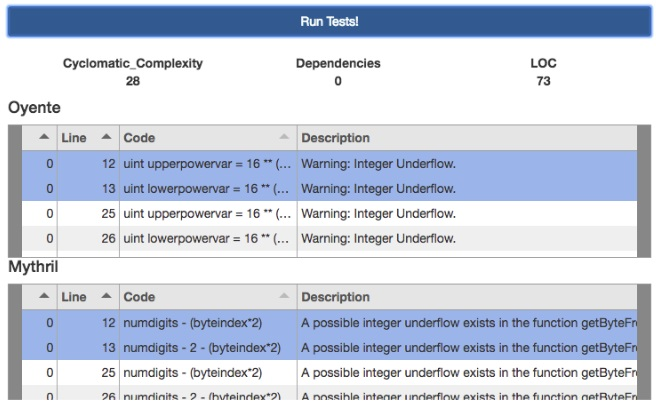
\includegraphics[width=0.5\textwidth]{img/ui2_2.jpg}
  \label{fig:ui2_2}
  \caption{The results of each test suite is highlighted to emphasize tagged code sections.}
\end{center}
\end{figure}

\subsection{User Interface}

To take advantage of the Mythril and Oyente testing suites, we present our user interface that allows running several testing applications and viewing the results interactively in a browser, shown in figure~\ref{fig:ui1}. Users can upload and modify or write a new Solidity Smart Contract in the syntax-highlighted editor, and choose to run Oyente, Mythril, SmartCheck or any combination of the three tools to detect security vulnerabilities in the code. The output is displayed as a verbose list of errors and warnings with exact line numbers identifying the cause of the vulnerability. \\

The application is a web based front-end that can run in any browser, supported by a Python back-end that automatically schedules tasks and prepares environments for each tool individually, reducing the amount of set-up time and knowledge required on behalf of the user to effectively nothing beyond loading a web-page. Additionally, the back-end is able to maintain the environment using docker containers to drastically speed up future runs of the test suites, reducing the overhead time and computational costs of each run after the first from the order of minutes to mere seconds. \\

\begin{figure}
\begin{center}
  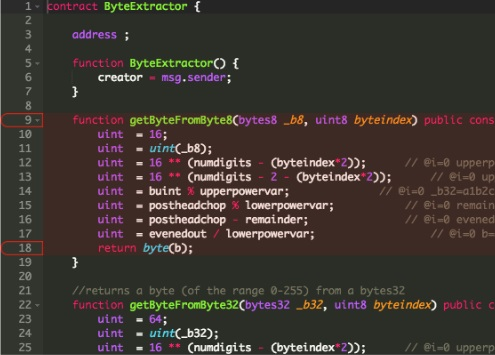
\includegraphics[width=0.5\textwidth]{img/ui2_1.jpg}
  \label{fig:ui2_1}
  \caption{A Smart Contract in the interface can be highlighted with the side-bar, shown here from lines 9 to 18.}
\end{center}
\end{figure}

The interface supports user-defined tagged sections for identifying critical sections of smart contracts. By highlighting, or "tagging," a section of the smart contract, a user can get more specific feedback from the test suites, shown in figure~\ref{fig:ui2_1}. This feature is currently limited to only prioritizing and clarifying information related to the tagged sections of code, shown in figure~\ref{fig:ui2_2}, but in the future could also influence the behavior of tools. For instance, if a tool is timing out while running analysis on the smart contract, we could ensure that it is prioritizing tagged sections and leaving less important sections to be possibly cut short. None of the tools we've tested in this work, however, face the issue of timing out while analyzing reasonable length smart contracts, so this feature would not be useful with the current implementation. \\

Portability and accessibility are achieved through Docker containers that are managed by the API. Each container has the necessary environment and dependencies, automatically fetching them from a trusted repository, so that even running locally, the tool requires minimal set-up. While it can be run locally, the application as a whole is intended to be used entirely web-based, uploading the Smart Contract to a remote server for testing and returning the results within a browser window. \\

Our solution covers several use cases, primarily those of the Smart Contract writer, the second party to a contract, as well as reviewers of the implemented test-suites. The Smart Contract writer is able to interactively view vulnerabilities in her code and quickly make iterative changes with the built-in and fully syntax-aware code editor window. The second party, assumed to be ignorant of the finer points of Smart Contracts, including how to write them, is able to verify security and integrity without having to learn from scratch how to run any of these complicated test suites on his own. Finally, a reviewer can take contracts with known or unknown flaws and compare the outputs of multiple tools to test which produces the best or most accurate output. \\

This user interface is designed and used not only for our study to measure the ability of Oyente, Mythril and SmartCheck to detect security flaws, but also for the public to use to have easily accessible testing capabilities for any Smart Contract written in Solidity. With this tool, testing a Solidity Smart Contract is easy and straightforward, since the entire process from fetching dependencies all the way to destroying the containers on completion is managed totally automatically. This end-to-end approach is intended to make it possible for a lay-person to engage in a Smart Contract knowing that it has been tested by the best open-source tools available, while still providing the important technical information that the contract writer needs to create a sound and error-free contract. \\

     
\begin{table*}[h!]
\centering
\begin{tabular}{|ccccccc|}
\hline
 & & \textbf{Cyclomatic Complexity}	&\textbf{Dependencies}&	LOC	&	\textbf{\# Errors} &	\textbf{\# Issues} \\

\hline
SmartCheck & Original  & 16.07 & 0.302 & 81.613   & 4.316 & \\
        & Mutated  & 44.249 & 0.444 & 81.613   & 5.348 & \\
 Oyente & Original   & 16.07 & 0.302 & 81.613  & 2.442 & 10.535\\
        & Mutated  & 44.249 & 0.444 & 81.613 &  5.026 & 0.9\\
Mythril & Original  & 16.07 & 0.302 & 81.613 &   0.977 & 5.767\\
        & Mutated  & 44.249 & 0.444 & 81.613 &   1.077 & 3.209\\
\hline
\end{tabular}\\
\label{tbl:Statistics}
\caption{ The statistical analysis of the different test suits for both the original and mutated scripts. This shows that SmartCheck detects the most bugs, followed by Oyente, and then Mythril. Moreover, this is much more pronounced with the mutated scripts. Note, SmartCheck did not provide meaningful warnings and thus has no associated Issues column.}
\end{table*} 

\subsection{Analysis Techniques}
\subsection*{Mutation Studies}
\begin{figure}[h!]
\lstinputlisting[language=C]{code/proposal.txt} 
\label{code:proposal}
\caption{Example script from the DAO smart contract codebase.}
\end{figure}
To expand upon the testing suites, we added mutations to the Solidity scripts to compare which suites would recognize that these perturbations. To create these mutations we replaced standard operations with contrary logic while avoiding syntactical errors. With these changes, we ran the testing suites again on the altered scripts. \\

The mutations were applied as a search and replace of a single operation per test. Thus, a file containing 10 unique operations would produce 10 mutated files each with a single operation mutated. For the mutations, we chose operations that would reverse the logic of the of the given statement. For example, consider the block of code from the DAO smart contract in Figure \ref{code:proposal}. \\

In this example, there is a list of checks that are made prior to scheduling a contract between a \texttt{sender} and \texttt{recipient}. Specifically, the receiving party is first checked against a list of allowed recipients, the debating period, or time frame to cancel the contract, is confirmed to be in a predefined range, that enough money has been deposited to cover this transaction, and importantly a check against a 51\% attack, where a majority owner of the block chain can cheat the system, is protected against. A valid testing suite should recognize the insecurities presented if any one of this statements is not checked. Thus our mutations primarily change the logic in checks like the one above. A simple way to guarantee this is by reversing the logic on each operation. For example the check against a 51\% attack relies on a equality constraint, thus if this changed to an inequality we can guarantee that check will fail. A complete list of the mutations made on each Solidity script is  given in table \ref{Mutations}. \\
     
\subsection*{Static Analysis}

In addition to Mutation studies, we also performed static analysis on the solidity scripts to provide metrics to help explain why one suite performed better than another. These metrics include measuring the number of lines, complexity, and dependencies in a block of code. These metrics were chosen following the results of Kochnar et al.'s code coverage study \cite{kochhar2017code}. \\

The statistical measures used to analysis the solidity script were Lines of Code (LOC), Cyclomatic Complexity, and the number of Dependencies. Lines of Code was directly computed from each script after removing whitespace and comments. One limitation of this measure, is that it does not account for varying coding styles, such as placing brackets in line with function signatures, but overall this provided a good metric for length of a script. Cyclomatic Complexity measure the dependence between certain paths within a block of code. This metric increases by one at each point where a new branch will need to be tested; such as an if statement or logical decision \cite{mccabe1976complexity}. Dependencies measures the number of imports into a script, causing this file to require correct execution of the dependent file. For example a DAO solidity package consists of many separate scripts that each import a base DAO class. Thus each of these would have a dependency of at least 1. With these measures, we were able to balance the testing suite results with concrete information that can easily be pulled from a script; allowing for breadth in our study. \\




\section{Results \& Analysis}
\subsection{Testing Comparison}

As part of our analysis, we created the SSCTT Web-based User Interface, and we use it drastically streamline the pipeline for running Solidity contract test suites. And while it still currently only supports Oyente and Mythril, we've already been able make full-fledged security vetting of smart contracts possible for any person regardless of skill level. While it is not in the scope of this paper, we intend to perform a user study and formal evaluation of our tool in the future. Even without this, however, the impact of moving these test suites from command-line tools to fully managed and contained web-apps is clear. Users are able to see prettified results in order of importance to them. Furthermore, the accessibility benefit of automating the set-up and tear-down of the existing tools is motivated by the need for uneducated parties to be able to verify their smart contracts' security. Thus, we consider the Web Interface a success in this regard. \\

\subsection{Mutation Tests}

Both suites provide very different results when trying to analyze a Solidity script. To understand the reason behind this, we employed a combination of mutation testing and static analysis methods. On average, each script had 9.27 operations that were mutated to produce a list of mutated scripts. Then each of the two suites were run on the original Solidity files and on each of the mutations. \\

Figure \ref{tbl:Statistics} shows a summary of the errors and issues found by each suite across our collection of solidity scripts. Here we see that Oyente found 83\% more issues than Mythril on the original document, and 153\% more errors on the mutated scripts. On average SmartCheck found more bugs than Oyente in both cases, but a large part of this can be attributed to the scripts with no bugs. In these cases, Smart Check continues to detect bugs; thus leading to many false positives. With larger scripts with many bugs, Oyente and Mythril significantly detect more bugs than SmartCheck. However, in general smart contracts are usually smaller, and define a very specific purpose of ensuring transactions are completed according to all parties. \\

\subsection{Static Analysis}

To study the suites in more detail, we plotted the number of bugs found by each suite (Figure \ref{bugs} Left, Middle). If each suite were exactly the same, then each point would lie on the $y=x$ line. However, in the first plot we see a consistent trend to the right of this line. This means that Oyente has found more bugs in every script than Mythril. For the middle plot, we perform the same comparison of Oyente and Smartcheck. For this comparison, we see a sections of tests where SmartCheck finds more bugs, and another section where Oyente does. On further inspection, SmartCheck finds more bugs on the smaller less buggy scripts; while Oyente is significantly better at detecting bugs in the larger more complicated scripts.  This trend is minimally impacted by mutations in the code, but for the Oyente vs. Mythril comparison it is clear that that Oyente outperforms Mythril on mutated scripts.\\

The plot to the right of Figure \ref{bugs} shows the number of bugs as a function of complexity of the script. Here we see a trend where scripts that are smaller and scripts that are larger tend to have more bugs. It is expected that a larger script would have more bugs, but scripts with average complexity have much less bugs than low complexity scripts.  SmartCheck breaks this trend by having many more bugs with the smaller scripts, and less with the larger scripts. A possible explanation for this is that smaller scripts tended to have significantly less error handling; thus bugs would be caught less. Moreover, SmartCheck tends to focus on bad error handling where the other suites ignore this altogether.  \\

\subsection{Specific Bugs}

Although quantity of bugs is important, specific bugs are responsible for the DAO attack and can cause insecurities in the contracts. Thus, focusing on the quality of the bugs is vital for smart contract testing suites. Specifically, we tested a smart contract that checks if a given any address is valid. For this contract, Oyente detects a possible integer underflow, SmartCheck states that one of the variables in the function could be private but was defined as public (\texttt{SOLIDITY\_VISIBILITY}), and Mythril provides a meaningful warning that having no validation on the input address allows for users to provide injection attacks using this function. For both Oyente and SmartCheck, their bugs offer no security vulnerabilities or possible solutions, while Mythril describes the specific threat and why it is a threat.  

Like previously mentioned, some of the vulnerabilities that we found were of high quality and very notable in the sense that they have previously been exploited to in famous hacks. For example, Mythril error-checks a contract by looking for inputs that trigger and unprotected SUICIDE or SELFDESTRUCT instruction. With this instruction, a smart contract is essentially destroyed and all the remaining balance of the contract to a specified address. This bug was famously revealed in November 2017, when an anonymous Github user "accidentally" became the owner of the main library contract and then proceeded to self-destruct it. Because he was successfully able to call an unprotected self-destruct instruction, about \$300 million was frozen and inaccessible forever. Presumably, had this contract been debugged using the Mythril test suite, this error would have been caught.  

Another such example comes from the highly publicized DAO attack. In the DAO attack, a hacker made use of a "reentrancy" bug to drain Ethereum from the DAO. Reentrancy attacks occur when the external contract called by the initial contract is allowed to make new calls to the calling contract before the initial execution is complete. In this way, an untrustworthy external contract can take advantage of the callee contract. Oyente looks for such reentrancy issues in contracts, once again showing the quality of the vulnerabilities we found. 

Furthermore, these findings also justify the need for our tool. Since Oyente, Mythril, and SmartCheck are implemented differently, they look for different types of issues. Therefore, to get the best coverage on your code, the use of multiple tools is highly encouraged. However, all of these tools run on different environment and are hard to find unless one is to search for them by name. Our tool is also easy to update - a test suite can easily be added. Therefore, we provide a useful, simple platform for a developer to take advantage of all the tools available to them.   

\begin{figure*}[h!]
\centering
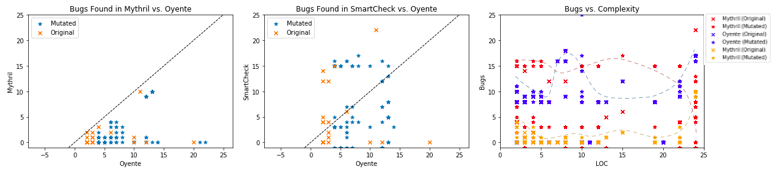
\includegraphics[width=7.0in]{img/Bugs2.png}
\caption{Plots of the number of bugs found with each suite (Left, Middle) and the number of bugs found as a function of the script's complexity (Right). Here we see that Oyente consistently detects more bugs than Mythril, but SmartCheck detects the most bugs of all suites. Moreover, the number of bugs does not increase monotonically in complexity, but is bimodal where lowest and highest complexity lead to more bugs.}
\label{bugs}
\end{figure*}


\section{Conclusion}

We noticed that the correlation between complexity and errors is not as expected. In general, a larger file with more complexity should have more bugs, but we found that the the smaller files had almost as many bugs as the largest files. Moreover, files with average complexity had the least number of bugs. We attribute this to there being less code in smaller files, so less error checking. Thus, the medium sized files have similar logic to files of lower complexity, but spend more lines of code to catch errors. \\

Moreover, after mutating the scripts, the number of bugs that Oyente found increased nearly 5 times, where Mythril and SmartCheck found nearly the same number of bugs on average. This can likely be attributed to the types of bugs that Mythril searches for. With chain execution, Mythril misses bugs related to bad operations as the paths remain relatively unchanged. Interestingly, Mythril found many more issues in the mutated scripts, providing credence to the idea that Mythril treats mutations differently from Oyente or SmartCheck. In conclusion, we find that the Oyente testing suite significantly more bugs than Mythril on most scripts, and more bugs than SmartCheck on complex scripts. In contrast, the Mythril tool provides more details of each bugs, and the SmartCheck focuses on vastly different bugs altogether. 

The focus of this experiment was to determine the quality of bugs, and Mythril appears to surpass both tools in this area. The bugs found by Oyente were primarily related to tasks such as integer overflow, and the primary bugs found by SmartCheck were \texttt{SOLIDITY\_VISIBILITY} bugs where a variable or function is public when it can be private. The Mythril suite found bugs associated to bad parameters that could be used as back doors for attacks, such as passing a raw address to a contract. Thus, although in many cases both Oyente and SmartCheck found more bugs, the Mythril suite finds better bugs.



\section{Future Work}

Currently, our tool uses Oyente, Mythril, and SmartCheck to analyze Solidity smart contracts, then reports the bugs found within. These three give us the widest coverage while maintaining accuracy. This succeeds in allowing Solidity developers in an easy-to-use interface and gives a variety of results. We also allow developers to flag certain code snippets to be more important. We have also expanded on our previous experiments by running on a wider variety of smart contracts. Two notable large contracts here (King of the Ether and Cryptokitties) are over 1,000 lines long. \\

Moving forward, we'd like to provide an easier method to allow updates for analyzers so they may easily adapt to future changes. Additionally, enabling developers to add their own testing suites would be useful as well. Since many smart contracts have similar crucial areas (e.g. authentication, external oracle, sending money, etc), perhaps we could recommend templates with secure design patterns to the developer depending on their code's errors. \\

For improving analysis tools, most tools often come up with false positive or negatives. Improving on accuracy would save time and developer effort. Furthermore, these tools are currently quite difficult to find. They are infrequently mentioned in official documentation and most new developers will not immediately think to look for these tools. As such, providing a Solidity IDE would be a promising way to quickly improve smart contract code quality, as they could embed testing suites by default. Overall, smart contracts have fantastic potential; improving code quality through better testing would quickly reduce the number of buggy contracts on the network, thus encouraging user growth!  



\bibliographystyle{ieeetr}
\bibliography{sections/bib.bib}
\end{document}
